\documentclass{article}

\usepackage{amsmath}
\usepackage{graphicx}
\usepackage{enumitem}

\title{Strata Filter}
\author{Guy John \\ \texttt{guy@rumblesan.com}}

\begin{document}

\maketitle

\section{Introduction}
Analysis of the Strata filter. Heavily based on the Serge VCFQ, but also with influence from the Mutable Instruments Blades. Much of this is pulled verbatim from the SSM2164 SVF Analysis by Emilie Gillet and then just somewhat modified.

\newpage

\subsection{Notations}

\begin{description}
\item $R_i$ is the value of the resistor through which the input signal is fed to the circuit.
\item $R_f$ is the value of the resistor through which the output signal of the integrator is fed back to the input.
\item $R_s$ is the value of the resistor from the OTA inputs to ground.
\item $C$ is the value of the integrators' capacitors.
\item $R_g$ is the value of the resistor through which the HP and LP outputs are fed back into the input.
\item $R_q$ is the value of the resistor through which the attenuated BP output is fed back into the input.
\item $v_{cv}$ is the cutoff frequency control voltage.
\item $v_q$ is the resonance control voltage.
\item $v_i(s)$ is the input voltage.
\item $v_{hp}(s)$, $v_{bp}(s)$ and $v_{lp}(s)$ are the high-pass, band-pass and low-pass output voltages.
\end{description}

\subsection{OTA Integrator Cell}

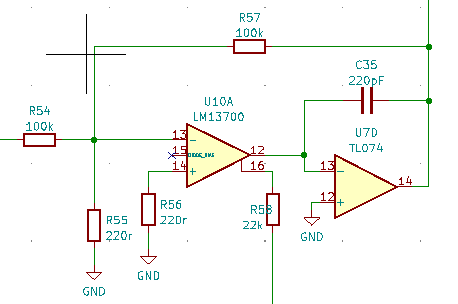
\includegraphics[width=\linewidth]{images/incorrect-otacell.png}

The transfer function of an OTA is:

\begin{equation*}
\begin{split}
  i_o & = g_m(v_+ - v_-) \\
  i_o & = 19.2i_{cv}(v_+ - v_-) \\
\end{split}
\end{equation*}

If $R_f$ is equal to $R_i$
Kirchoff in $v_-$ gives:

\begin{equation*}
\begin{split}
  \frac{1}{R_i}(v_i(s) - v_-(s)) + \frac{1}{R_i}(v_{out}(s) - v_-(s)) & = \frac{1}{R_s}v_-(s) \\
  {R_s}v_i(s) - {R_s}v_-(s) + {R_s}v_{out}(s) - {R_s}v_-(s) & = {R_i}v_-(s) \\
  {R_s}v_i(s) + {R_s}v_{out}(s) - {R_s}v_-(s) - {R_s}v_-(s) & = {R_i}v_-(s) \\
  {R_s}v_i(s) + {R_s}v_{out}(s) - 2{R_s}v_-(s) & = {R_i}v_-(s) \\
  {R_s}v_i(s) + {R_s}v_{out}(s) & = {R_i}v_-(s) + 2{R_s}v_-(s) \\
  {R_s}(v_i(s) + v_{out}(s)) & = v_-(s)({R_i} + 2{R_s}) \\
  \frac{R_s}{{R_i} + 2{R_s}}(v_i(s) + v_{out}(s)) & = v_-(s) \\
\end{split}
\end{equation*}

The current $i_c$ at the output if the OTA is:

\begin{equation*}
\begin{split}
  i_c(s) & = g_m(v_+(s) - v_-(s)) \\
   & = 19.2i_{cv}(0 - \frac{R_s}{{R_i} + 2{R_s}}(v_i(s) + v_{out}(s))) \\
   & = -19.2i_{cv}\frac{R_s}{{R_i} + 2{R_s}}(v_i(s) + v_{out}(s)) \\
\end{split}
\end{equation*}

The voltage out of the OpAmp:

\begin{equation*}
\begin{split}
  v_{out}(s) & = \frac{-i_c(s)}{Cs} \\
  v_{out}(s) & = -(-19.2i_{cv}\frac{R_s}{Cs({R_i} + 2{R_s})}(v_i(s) + v_{out}(s))) \\
  v_{out}(s) & = 19.2i_{cv}\frac{R_s}{Cs({R_i} + 2{R_s})}(v_i(s) + v_{out}(s)) \\
  v_{out}(s)Cs({R_i} + 2{R_s}) & = 19.2i_{cv}R_s(v_i(s) + v_{out}(s)) \\
  v_{out}(s)Cs({R_i} + 2{R_s}) & = v_i(s)19.2i_{cv}R_s + v_{out}(s)19.2i_{cv}R_s \\
  v_{out}(s)Cs({R_i} + 2{R_s}) - v_{out}(s)19.2i_{cv}R_s & = v_i(s)19.2i_{cv}R_s \\
  v_{out}(s)(Cs({R_i} + 2{R_s}) - 19.2\i_{cv}R_s) & = v_i(s)19.2i_{cv}R_s \\
  v_{out}(s) & = v_i(s)\frac{19.2i_{cv}R_s}{Cs({R_i} + 2{R_s}) - 19.2i_{cv}R_s} \\
  v_{out}(s) & = v_i(s)\frac{1}{\frac{({R_i} + 2{R_s})}{R_s}Cs\frac{1}{19.2i_{cv}} - 1} \\
\end{split}
\end{equation*}

So the transfer function is:

\begin{equation}
  \alpha(s) = \frac{1}{\frac{({R_i} + 2{R_s})}{R_s}Cs\frac{1}{19.2i_{cv}} - 1}
\end{equation}

This should work as a single filter stage in itself, with the cutoff frequency being the point at which the ouput is 3dB lower than the input, or $\frac{1}{\sqrt{2}} \approx 0.707$

\begin{equation*}
\begin{split}
  0.707 & = \frac{1}{\frac{({R_i} + 2{R_s})}{R_s}C2\pi{f}\frac{1}{19.2i_{cv}} - 1} \\
  0.707\frac{({R_i} + 2{R_s})}{R_s}C2\pi{f}\frac{1}{19.2i_{cv}} -  0.707 & = 1 \\
  0.707\frac{({R_i} + 2{R_s})}{R_s}C2\pi{f}\frac{1}{19.2i_{cv}} & = 1.707 \\
  \frac{({R_i} + 2{R_s})}{R_s}C2\pi{f}\frac{1}{19.2i_{cv}} & = \frac{19.2i_{cv}1.707}{0.707} \\
  f\frac{({R_i} + 2{R_s})}{R_s}C2\pi & = 19.2i_{cv}2.414 \\
  f & = \frac{19.2i_{cv}2.414}{2\pi\frac{({R_i} + 2{R_s})}{R_s}C} \\
  f & = \frac{19.2i_{cv}1.207}{\pi\frac{({R_i} + 2{R_s})}{R_s}C} \\
  f & = \frac{23.18i_{cv}}{\pi\frac{({R_i} + 2{R_s})}{R_s}C} \\
\end{split}
\end{equation*}

\subsection{Feedback Control}

The gain of the feedback circuit is:

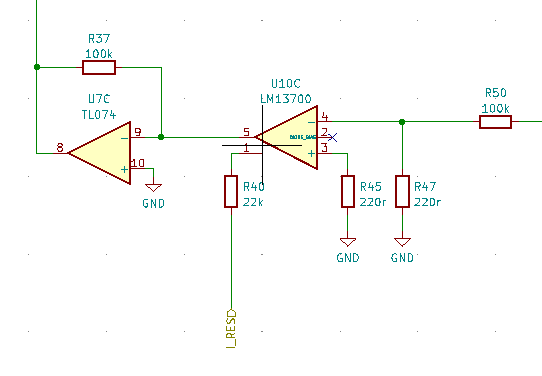
\includegraphics[width=\linewidth]{images/feedback-amp.png}

\begin{equation*}
\begin{split}
  v_- & = v_i\frac{R_s}{R_i + R_s} \\
  i_o & = 19.2i_{res}(0 - v_-) \\
  i_o & = -19.2i_{res}v_i\frac{R_s}{R_i + R_s} \\
  i_o + \frac{v_o}{R_f} & = 0 \\
  i_o & = -\frac{v_o}{R_f} \\
  -i_o{R_f} & = v_o \\
  v_o & = -i_o{R_f} \\
  v_o & = 19.2i_{res}v_i\frac{R_fR_s}{R_i + R_s} \\
  v_o & = 19.2i_{res}v_i\frac{R_fR_s}{R_i + R_s} \\
  \beta & = 19.2i_{res}\frac{R_fR_s}{R_i + R_s} \\
\end{split}
\end{equation*}

\subsection{Filter}

\begin{equation*}
\begin{split}
  \frac{v_i - v_-}{R_i} + \frac{v_{hp} - v_-}{R_f} + \frac{v_{lp} - v_-}{R_f}  + \frac{v_{bp}\beta - v_-}{R_q} & = i_- = 0 \\
  \frac{v_i}{R_i} + \frac{v_{hp}}{R_f} + \frac{v_{lp}}{R_f}  + \frac{v_{bp}\beta}{R_q} & = 0 \\
\end{split}
\end{equation*}

It is important to note that $v_{bp}(s) = v_{hp}(s)\alpha(s)$, and $v_{lp}(s) = v_{hp}(s)\alpha(s^2)$.

\subsubsection{High-pass}

\begin{equation*}
\begin{split}
  \frac{v_{hp}(s)}{R_f} & = - \frac{v_i(s)}{R_i} - \frac{v_{lp}(s)}{R_f} - \frac{v_{bp}(s)\beta}{R_q} \\
  \frac{v_{hp}(s)}{R_f} & = - \frac{v_i(s)}{R_i} - \frac{v_{hp}(s)\alpha(s^2)}{R_f} - \frac{v_{hp}(s)\alpha(s)\beta}{R_q} \\
  H_{hp}(s) & = \frac{v_{hp}(s)}{v_i(s)} \\
  \frac{v_i(s)}{R_i} & = - \frac{v_{hp}(s)}{R_f} - \frac{v_{hp}(s)\alpha(s^2)}{R_f} - \frac{v_{hp}(s)\alpha(s)\beta}{R_q} \\
  \frac{v_i(s)}{R_i} & = - v_{hp}(s)(\frac{1}{R_f} + \frac{\alpha(s^2)}{R_f} + \frac{\alpha(s)\beta}{R_q}) \\
  \frac{1}{R_i} & = - H_{hp}(s)(\frac{1}{R_f} + \frac{\alpha(s^2)}{R_f} + \frac{\alpha(s)\beta}{R_q}) \\
  \frac{-1}{R_i} & = H_{hp}(s)(\frac{1}{R_f} + \frac{\alpha(s^2)}{R_f} + \frac{\alpha(s)\beta}{R_q}) \\
  H_{hp}(s) & = \frac{-1/R_i}{\frac{1}{R_f} + \frac{\alpha(s^2)}{R_f} + \frac{\alpha(s)\beta}{R_q}} \\
  & = \frac{-R_f/R_i}{1 + \frac{R_f\alpha(s)\beta}{R_q} + \alpha(s^2) } \\
\end{split}
\end{equation*}

\subsubsection{Low-Pass}

\begin{equation*}
\begin{split}
  H_{lp}(s) & = \frac{v_{lp}(s)}{v_i(s)} \\
            & = \frac{v_{hp}(s)}{v_i(s)}\alpha^2(s) \\
            & = \frac{-}{\frac{1}{\alpha^2(s)} + \frac{R_f\beta}{R_q\alpha(s)} + 1 } \\
            & = \frac{-R_f/R_i}{\frac{1}{\alpha^2(s)} + \beta\frac{R_f}{R_q}\frac{1}{\alpha(s)} + 1 } \\
            & = \frac{-R_f/R_i}{\frac{1}{(\frac{1}{\frac{{R_i} + 2{R_s}}{R_s}Cs\frac{1}{19.2i_{cv}} - 1})^2} + (19.2i_{res}\frac{R_fR_s}{R_i + R_s})\frac{R_f}{R_q}\frac{1}{(\frac{1}{\frac{{R_i} + 2{R_s}}{R_s}Cs\frac{1}{19.2i_{cv}} - 1})} + 1 } \\
            & = \frac{-R_f/R_i}{(\frac{{R_i} + 2{R_s}}{R_s}Cs\frac{1}{19.2i_{cv}} - 1)^2 + (19.2i_{res}\frac{R_fR_s}{R_i + R_s})\frac{R_f}{R_q}(\frac{{R_i} + 2{R_s}}{R_s}Cs\frac{1}{19.2i_{cv}} - 1) + 1 } \\
            & = \frac{-R_f/R_i}{(\frac{{R_i} + 2{R_s}}{R_s}Cs\frac{1}{19.2i_{cv}})^2 - 2(19.2i_{res}\frac{R_fR_s}{R_i + R_s}) + 1 + (19.2i_{res}\frac{R_fR_s}{R_i + R_s}\frac{R_f}{R_q})(\frac{{R_i} + 2{R_s}}{R_s}Cs\frac{1}{19.2i_{cv}} - 1) + 1 } \\
            & = \frac{-R_f/R_i}{(\frac{{R_i} + 2{R_s}}{R_s}Cs\frac{1}{19.2i_{cv}})^2 - (2 + \frac{R_f}{R_q})(19.2i_{res}\frac{R_fR_s}{R_i + R_s}) + 19.2i_{res}\frac{R_fR_s}{R_i + R_s}\frac{R_f}{R_q}\frac{{R_i} + 2{R_s}}{R_s}Cs\frac{1}{19.2i_{cv}} + 2 } \\
            & = \frac{-R_f/R_i}{(\frac{{R_i} + 2{R_s}}{R_s}Cs\frac{1}{19.2i_{cv}})^2 + 19.2i_{res}\frac{R_fR_s}{R_i + R_s}\frac{R_f}{R_q}(\frac{{R_i} + 2{R_s}}{R_s}Cs\frac{1}{19.2i_{cv}}) - (2 + \frac{R_f}{R_q})(19.2i_{res}\frac{R_fR_s}{R_i + R_s}) + 2 } \\
\end{split}
\end{equation*}

At this point it seems clear that this doesn't fit the standard transfer function for a second order filter....

\end{document}
